\documentclass[13pt, t]{beamer}

% Presento style file
\usepackage{config/presento}

% custom command and packages
% custom packages
\usepackage{textpos}
\setlength{\TPHorizModule}{1cm}
\setlength{\TPVertModule}{1cm}

\newcommand\crule[1][black]{\textcolor{#1}{\rule{2cm}{2cm}}}



% Information
\title{\Large \hspace{-0.5cm} The speakers of minority languages  \textbf{are more multilingual}}
\author[shortname]{Nina Dobrushina and George Moroz\bigskip}
\institute[shortinst]{Linguistic Convergence Laboratory, NRU HSE, Moscow, Russia}
\date{\begin{center} 16 April 2019 \bigskip \\ {{\color{colorblue} \href{https://ilcl.hse.ru/smallscale/}{\large Typology of small-scale multilingualism} \\ Laboratoire Dynamique du Langage, Lyon, France }\\ \vfill Presentation is availible here: \href{tinyurl.com/y6jjp38y}{\large \color{colorblue}  \textbf{tinyurl.com/y6jjp38y} \hfill 
\includegraphics[height = 2.5cm]{images/01_qrcode}}} \end{center}}

\begin{document}

% Title page
\begin{frame}[plain]
\maketitle
\end{frame}

\framecard[colorblue]{{\color{colorwhite} \huge Problem part}}

\framecard[colorblue]{{\color{colorwhite} \huge Data}}
\begin{frame}{Data}
Data obtained during interviews on language usage from about 15 fieldtrips (see \citep{dobrushina2013} for methodology details) and  collected into \textbf{Atlas of Multilingualism in Daghestan} \citep{multidagestan17}:
\begin{itemize}
\item 46 Daghestanian villages
\item 24 langugages (Russian excluded) \pause
\item 29 860 people born between 1900 and 1959
\begin{itemize}
\item 14 410  females (48.2\%)
\item 15 450 males (51.7\%)
\end{itemize}
\item variable containing number of known languages\pause
\item we grouped all villages into three categories according to the nowaday number of speakers
\begin{itemize}
\item {\Large \color{colorbig} \textbf{big}} --- 100 000 speakers and more
\item {\Large \color{colormedium} \textbf{medium}} --- 10 000--30 000 speakers
\item {\Large \color{colorsmall} \textbf{small}} --- one village languages, 1 000--2 000 speakers
\end{itemize}
\end{itemize}
\end{frame}

\framepic{images/03_map_930_700}

\framepic{images/04_map_class_930_700}

\framepic{images/05_map_1900_930_700}

\framepic{images/06_map_1910_930_700}

\framepic{images/07_map_1920_930_700}

\framepic{images/08_map_1930_930_700}

\framepic{images/09_map_1940_930_700}

\framepic{images/10_map_1950_930_700}

\framepic{images/11_panel_1100_750}

\begin{frame}{Median number of L2 in each village by decade and language category}
\hspace{-0.9cm}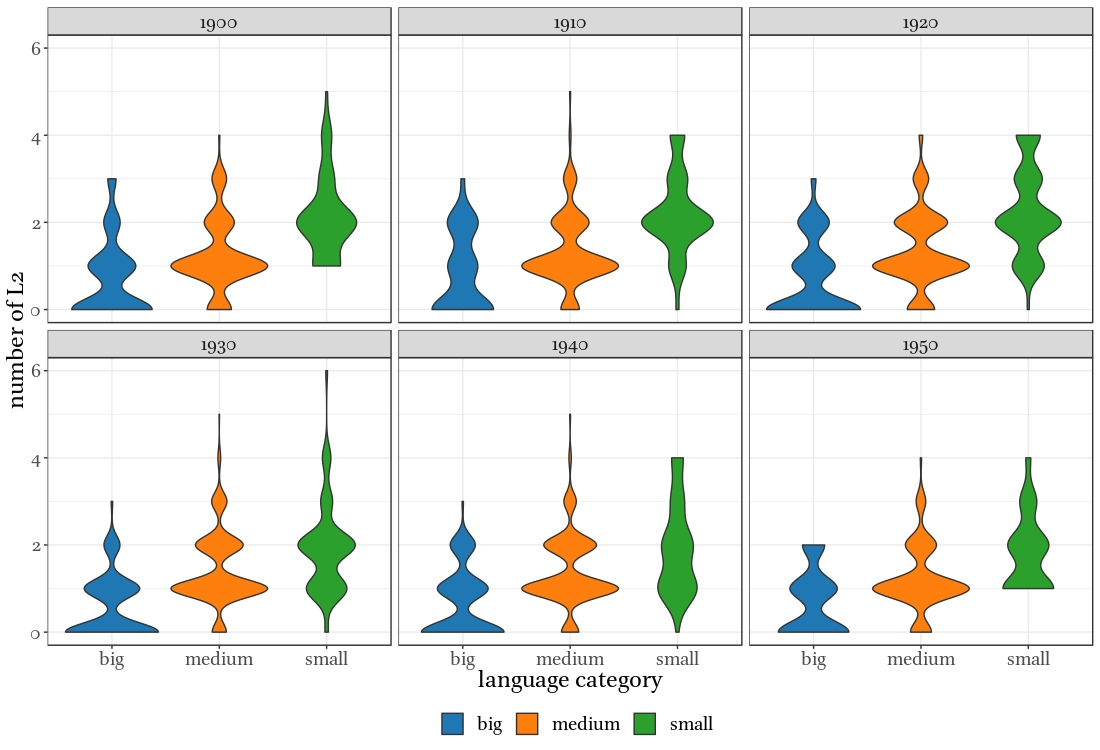
\includegraphics[width=1.08\linewidth]{images/12_panel_1100_750}
\end{frame}

\begin{frame}{Poisson Mixed Effects Model}
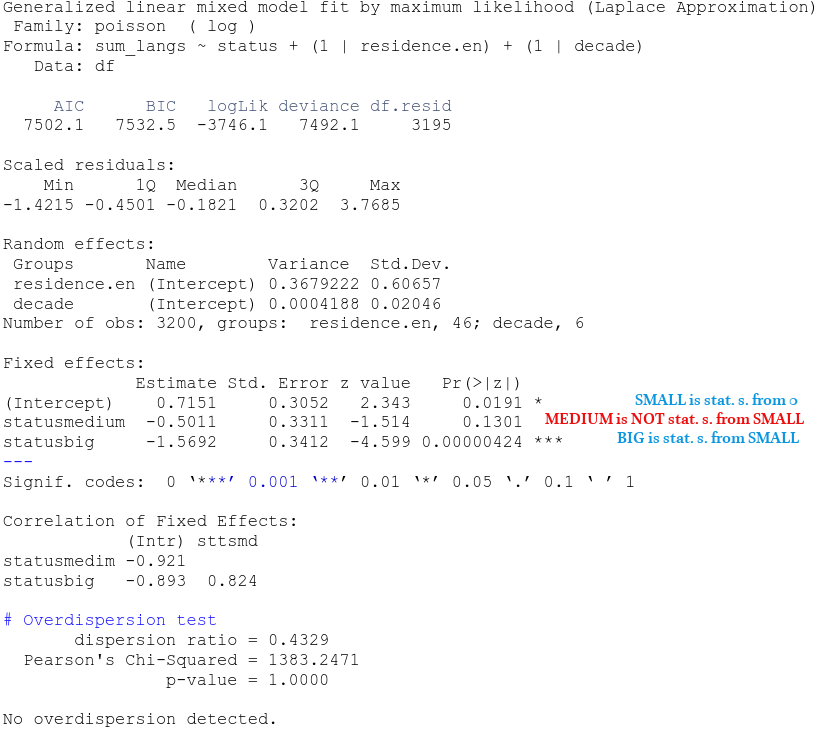
\includegraphics[width=0.87\linewidth]{images/13_poisson}
\end{frame}

\begin{frame}{Poisson Mixed Effects Model: Residuals}
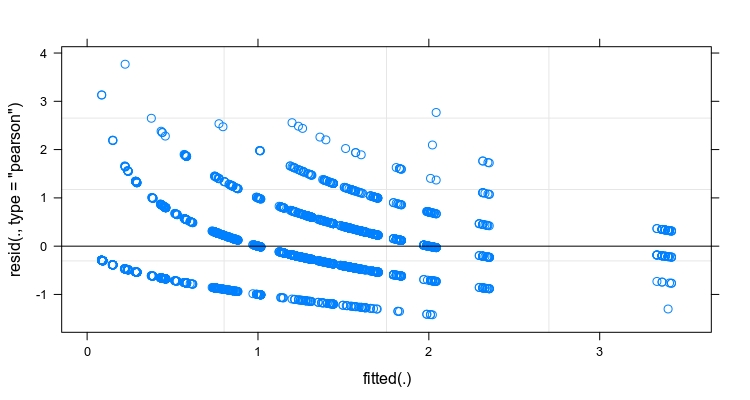
\includegraphics[width=\linewidth]{images/14_poisson_residuals_750_400}
\end{frame}

\begin{frame}{Conclussions:}
\begin{itemize}
\item The variable language size is statistically signifficant.
\item Obtained coefficients could be interpret as following:\\
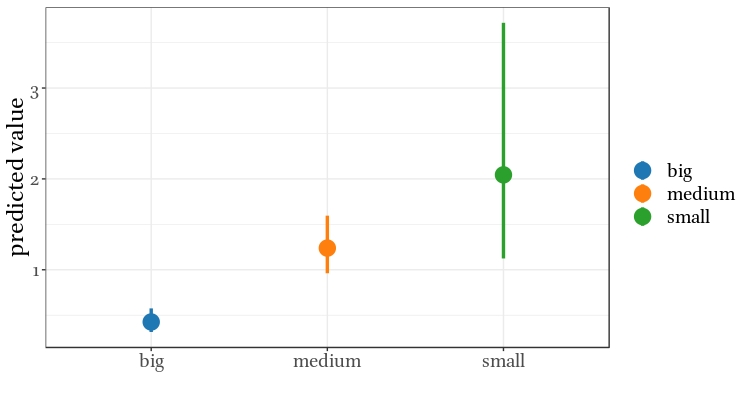
\includegraphics[width=\linewidth]{images/15_predicted_750_400}
\item Special case: Chuni
\end{itemize}
\end{frame}

\framecard[colorblue]{{\color{colorwhite} \Large Send us a letter!\\
nina.dobrushina@gmail.com\\
agricolamz@gmail.com\\ 
\vfill Presentation is availible here: \href{tinyurl.com/y6jjp38y}{\textbf{tinyurl.com/y6jjp38y}}\\
\vfill  
\includegraphics[height = 3cm]{images/02_qrcode}}\\
\vfill {\small  \color{colorwhite} All visualisation and statistical analysis were made in \texttt{R}~version~3.5.3~\citep{r19} with packages \texttt{ggplot2}~\citep{wickham16}, \texttt{lingtypology}~\citep{moroz17}, \texttt{lme4}~\citep{bates15}}}

%\begin{frame}[allowframebreaks]{Список литературы}
\begin{frame}{References}
\footnotesize
\bibliographystyle{config/chicago}
\bibliography{bibliography}
\end{frame}

\end{document}